\documentclass{beamer}

\usepackage[utf8]{inputenc}
\usepackage[T1]{fontenc}

\usepackage[english]{babel}
\usepackage{amsmath}
\usepackage{cleveref}
\usepackage{amssymb}
\usepackage{mathtools}

%%Numbers, expectation
\newcommand{\N}{\mathbb{N}}
\newcommand{\E}{\mathbb{E}}
\renewcommand{\P}{\mathbb{P}}
\newcommand{\Var}{\mathbb{V}}
\newcommand{\R}{\mathbb{R}}
\newcommand{\D}{\mathcal{D}}
\newcommand{\B}{\mathcal{B}}
\newcommand{\Dh}{\D_h}
\renewcommand{\phi}{\varphi}
\newcommand*\diff{\mathop{}\!\mathrm{d}} % integral

%% mathoperator
\DeclareMathOperator*{\argmax}{arg\,max}
\DeclareMathOperator*{\argmin}{arg\,min}
\DeclareMathOperator*{\dom}{dom}
\DeclareMathOperator*{\sign}{sign}
\DeclareMathOperator*{\diag}{diag}

\DeclareMathOperator*{\Cov}{Cov}
\DeclareMathOperator*{\Cor}{Corr}
\DeclareMathOperator*{\Id}{Id}

%proximal operator
\newcommand{\prox}[3][]{\operatorname{prox}^{#1}_{#2}\left(#3 \right)}

\usepackage{xcolor}

%% sort citations by increasing number
\usepackage[sort,nocompress]{cite}

\usepackage{graphicx}% http://ctan.org/pkg/graphicx
\graphicspath{{../figures/}{../../figures}{../../memes}} %Setting the graphicspath
\usepackage{caption,subcaption}

\usepackage{tikz}
\usepackage{pgfplots}
\usetikzlibrary{backgrounds}
\usetikzlibrary{intersections}
\usepgfplotslibrary{fillbetween}

% \usepackage[right]{showlabels}


%%
\theoremstyle{plain}
\newtheorem{prop}{Proposition}[section]
\newtheorem{algo}{Algorithm}[section]
\newtheorem{assumption}{Assumption}
\theoremstyle{remark}
\newtheorem{remark}{Remark}[section]

% cref
\crefname{assumption}{Assumption}{Assumptions}
\crefname{equation}{}{}

\usepackage{autonum}

\usepackage{bm} %% bold math symbols

\usepackage{bbm} %% for \mathbbm{1}


% algorithmic environment
\usepackage{algorithm}
\usepackage[noend]{algpseudocode}

% for some reason this was required on one void linux installation (but not the other)
\usepackage{sansmathaccent}
\pdfmapfile{+sansmathaccent.map}

\author{Axel Böhm}

% shows which section we're in
\usetheme{Darmstadt}

% page number
\setbeamertemplate{footline}[frame number]
\setbeamercolor{page number in head/foot}{fg=gray}


% display things like onslide or visible already before but grayed out
\setbeamercovered{transparent}

% set the itemize item symbol as a diamond
\setbeamertemplate{itemize item}{$\diamond$}
% set the itemize subitem symbol as a triangle
\setbeamertemplate{itemize subitem}{$\blacktriangleright$}

% set the enumerate item symbol as a roman numbers
\setbeamertemplate{enumerate item}{(\roman{enumi})}


\author{Axel Böhm}

% shows which section we're in
\usetheme{Darmstadt}

% page number
\setbeamertemplate{footline}[frame number]
\setbeamercolor{page number in head/foot}{fg=gray}


% display things like onslide or visible already before but grayed out
\setbeamercovered{transparent}

% set the itemize item symbol as a diamond
\setbeamertemplate{itemize item}{$\diamond$}
% set the itemize subitem symbol as a triangle
\setbeamertemplate{itemize subitem}{$\blacktriangleright$}

% set the enumerate item symbol as a roman numbers
\setbeamertemplate{enumerate item}{(\roman{enumi})}

\DeclareMathOperator*{\perm}{perm}

\title{Matrix scaling}

\begin{document}
\maketitle
\frame{\tableofcontents}

\section{Introduction}%

\begin{frame}
  \frametitle{Introduction}
  \textbf{given:} a matrix $A \in \R^{m\times n}_{\ge0}$, vectors $r \in \R_{>0}^m$ and $c \in \R^n_{>0}$\\
  \textbf{find:} nonneg.\ diagonal matrices $X$ and $Y$ such that for
  \begin{equation}
    B = XAY
  \end{equation}
  it holds that:
  \begin{equation}
    B \mathbbm{1}_n = r \quad \text{and} \quad B^T \mathbbm{1}_m = c
  \end{equation}
  where $\mathbbm{1}_n = (1, \dots, 1)$ exactly $n$-times.
  Equivalently
  \begin{equation}
    \Vert B_{i,:} \Vert_1 = r_i \quad \text{and} \Vert B_{:, j} \Vert = c_j.
  \end{equation}

  \begin{block}{}
    \centering
    In this case $A$ is called $(r,c)$-scalable.
  \end{block}
  \onslide<2->{%
    If $\Vert r \Vert_1 \neq \Vert c \Vert_1$ this is not possible.
  }
\end{frame}

\begin{frame}
  \frametitle{Visualization of diagonal scaling}

  \begin{equation}
    \begin{aligned}
    B = \begin{bmatrix}
      x_1 & & & \\
      & x_2 & & \\
      & & \ddots & \\
      & & & x_m
    \end{bmatrix}
    A
    \begin{bmatrix}
      y_1 & & & \\
      & y_2 & & \\
      & & \ddots & \\
      & & & y_n
    \end{bmatrix}
    \\
    =
    \begin{bmatrix}
      a_{1,1}x_1y_1 & a_{1,2}x_1y_2 & \cdots & a_{1,n} x_1y_m \\
      \vdots   & \ddots & & \\
      a_{m,1}x_m y_1 & & \cdots & a_{m,n}x_m y_m
    \end{bmatrix}
    \end{aligned}
  \end{equation}
  \begin{block}{\textbf{Application:} Ill conditioned linear system $Az = b$.}
    Can multiply both sides by $X$  and substitute $z= Yv$ to get instead
    \begin{equation}
      XAY v = X b
    \end{equation}
  \end{block}
\end{frame}

\section{Matchings}%
\label{sec:}

\begin{frame}
  \frametitle{$(0-1)$ matrices | bipartite graphs}
  \begin{minipage}{0.5\textwidth}
    \begin{equation}
      \begin{bmatrix}
        0 & 1 & 1 \\
        1 & 0 & 0 \\
        0 & 1 & 1
      \end{bmatrix}
    \end{equation}
  \end{minipage}
  \begin{minipage}{0.35\textwidth}
    \begin{figure}[ht]
      \centering
      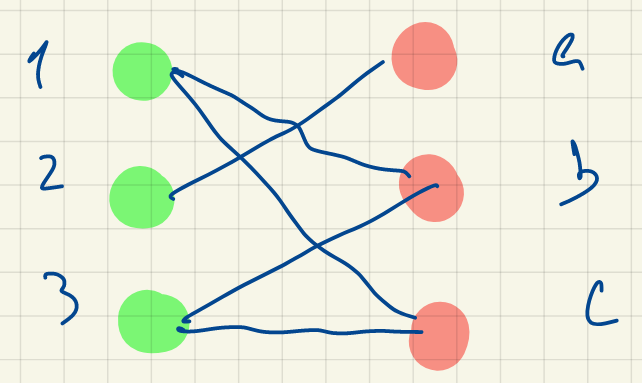
\includegraphics[width=\textwidth]{bipartite-graph.png}
      \caption{bipartite graph}
    \end{figure}
  \end{minipage}

    \begin{definition}
      \begin{itemize}
        \item A \textbf{matching} is a set of edges without common vertices.
        \item A \textbf{perfect matching} is a matching which covers all vertices.
      \end{itemize}
    \end{definition}
    Applications:
    \begin{itemize}
      \item marriage problem
      \item Hitchcock transport problem
    \end{itemize}
\end{frame}

\begin{frame}
  \frametitle{Finding the number of perfect matchings}
  Finding one is easy (polynomial time).
  Finding all is in \# P (i.e.\ hard!).
  \begin{block}{Consider $m=n$, $A\in \R^{n \times n}$}
    Recall:
    \begin{equation}
      \begin{aligned}
        &\text{(determinant)} \quad \det A = \sum_{\sigma} \sign(\sigma) \prod_{i=1}^n a_{i,\sigma(i)}  \\
        &\text{(permanent)} \quad \perm A = \sum_{\sigma} \prod_{i=1}^n a_{i,\sigma(i)}
      \end{aligned}
    \end{equation}
  \end{block}
  \begin{block}{Observation}
    For a $(0,1)-$matrix $A$, $\perm A$ is the number of perfect matchings.
    % This means that computing permanent must be hard.
  \end{block}
  One is easy to compute the other one hard. How can this be?
  % Diagionalize via gaussion elimination gives O(n^3) algorithm for computing determinant.
  % This doesn't work for permanent because it is not invariant under these operation (not multilinear).
\end{frame}

\section{Permanent}%
\label{sec:}

\begin{frame}
  \frametitle{Lower bounding the permanent}
  % This notion also appears in optimal transport
  \begin{definition}
    A matrix $A \in \R^{m\times n}_{\ge0}$ is called \textbf{doubly stochastic}, if sum of every row and every column is $1$.
  \end{definition}

  \begin{block}{van der Waerden (1926) conjectured}
    For doubly stochastic matrices the following \emph{lower bound} holds
    \begin{equation}
      \perm A \ge \frac{n!}{n^n}.
    \end{equation}
  \end{block}
  \begin{equation}
   \text{Is tight for } A = \begin{bmatrix}
      1/n & \cdots & 1/n \\
      \vdots & \ddots & 1/n \\
      1/n & \dots & 1/n
    \end{bmatrix}
  \end{equation}
  Proved in 1980.
\end{frame}


\begin{frame}
  \frametitle{Matrix scaling to approximate the permanent}
  \begin{block}{}
    If a $(0, 1)$-matrix $A$ can be scaled to be doubly stochastic, i.e.\ it is $\left(\mathbbm{1}, \mathbbm{1}\right)$-scalable, then
    we can apply lower bound
    \begin{equation}
      \perm B = \perm (XAY) = \left(\prod_i x_i\right) \left(\prod_j y_j\right) perm A
    \end{equation}
  \end{block}
\end{frame}

\begin{frame}
  \frametitle{Matrix scaling as an optimization problem}
  \begin{itemize}
    \item \textbf{given:} $A, r, c$
    \item \textbf{find:} $X, Y$ such that $B=XAY$ fulfills $B\mathbbm{1}_m=r$ and $B \mathbbm{1}_n=c$.
    \item $m+n$ unknowns
          \item $m+n$ constraints
  \end{itemize}
  Consider the (\emph{nonconvex}) function
  \begin{equation}
    g(x,y) = \langle x, A y \rangle - \langle r, \log x \rangle - \langle c, \log y \rangle
  \end{equation}
  with derivative (coordinatewise)
  \begin{equation}
    \label{eq:grad-original-formulation}
    \begin{aligned}
      \nabla_x g(x,y) = Ay - \frac{r}{x} \\
      \nabla_y g(x,y) = A^T x - \frac{c}{y}.
    \end{aligned}
  \end{equation}
\end{frame}


\begin{frame}
  \frametitle{Reparametrizing this system}
  Via reparametrization $x= e^\xi$ and $y=e^{\eta}$ we get
  \begin{equation}
    f(\xi, \eta) = \sum_{i,j} a_{i,j} e^{\xi_i + \eta_j} - \langle r, \xi \rangle - \langle c, \eta \rangle
  \end{equation}
  which is \textbf{\emph{convex}}. It's gradient is given by
  \begin{equation}
    \label{eq:grad-convex-reformulation}
    \frac{\partial f}{\partial \xi_i} = \sum_{j=1}^{n} a_{i,j} e^{\xi_i + \eta_j} - r_i
  \end{equation}
  Easy to see that the optimality condition of~\eqref{eq:grad-convex-reformulation} and~\eqref{eq:grad-original-formulation} agree.\\
  $\Rightarrow$ the nonconvex function only has \emph{global} minimizers.
\end{frame}

\begin{frame}
  \frametitle{Matrix scaling as an optimization problem [contd]}
  It is easy to see that a solution $(x,y)$ of
  \begin{equation}
    \begin{aligned}
      Ay - \frac{r}{x} = 0 \\
      A^T x - \frac{c}{y} = 0
    \end{aligned}
  \end{equation}
  defines a solution to the \emph{matrix scaling} problem via $X=\diag x$ and $Y=\diag y$
  \begin{equation}
    \left(\begin{array}{c}
            a_{1 1} y_1 + a_{1 2} y_2 + \cdots \\
            a_{2 1} y_1 + a_{2 2} y_2 + \cdots \\
            a_{m 1} y_1 + a_{m 2} y_2 + \cdots \\
          \end{array}\right)
        \begin{array}{c}
          \cdot x_1 = r_1\\
          \cdot x_2 = r_2\\
          \cdot x_m = r_m
        \end{array}
      \end{equation}
\end{frame}

\begin{frame}
  \frametitle{}
  The question remains: how to minimize
  \begin{equation}
    g(x,y) = \langle x, A y \rangle - \langle r, \log x \rangle - \langle c, \log y \rangle
  \end{equation}
  \vspace{-0.5cm}
  \begin{block}{alternating minimization}
    Given a problem
    \begin{equation}
      \min_{x,y} \phi(x,y)
    \end{equation}
    repeat:
    \begin{align}
      x_{k+1} &= \argmin_x \phi(x,y_k) \\
      y_{k+1} &= \argmin_y \phi(x_{k+1}, y).
    \end{align}
  \end{block}
    Makes sense as long as the \textcolor{blue}{subproblems are easy} (e.g. convex).
  \begin{align}
    &\text{opt. cond.\ for $x$:} \quad Ay - \frac{r}{x} = 0 \\
    &\text{opt. cond.\ for $y$:} \quad A^T x - \frac{c}{y} = 0
  \end{align}
\end{frame}


% change this to algorithmx package
\begin{frame}
  \frametitle{Sinkhorn's Algorithm}

  \begin{block}{Sinkhorn '60}
    Given $(x_0, y_0)$, for $k=1,\dots$
    \begin{equation}
      \begin{aligned}
        x_{k+1}&= \frac{r}{A y_k} \\
        y_{k+1}&= \frac{c}{A x_{k+1}} \\
      \end{aligned}
    \end{equation}
  \end{block}
  Linear convergence if $a_{i,j} > 0$.
  \textbf{Q:} What if $A$ is not $(r,c)$-scalable?
  % Then the optimization problem has no solution as FOC are never fulfilled
\end{frame}

\end{document}
